\chapter{Analyse}\label{k_analyse}

% Beschreibung des Aufbaus
\section{Versuchsaufbau}

Der Versuchsaufbau besteht aus einer drehbaren Scheibe mit Loch und einer Kugelabwurfvorrichtung.
Diese wird mit einem Servo bedient (siehe Abschnitt \ref{subs:aktoren}).
Abbildung \ref{img:versuchsaufbau} zeigt eine schematische Darstellung.
Da das Ziel des Praktikums ist, Kugeln durch das Loch fallen zu lassen, ist die Abwurfvorrichtung so angebracht, dass die Kugeln bei einer bestimmten Position der Scheibe durch dieses fallengelassen werden können.
Die Unterseite des Scheibe besitzt zwei Farbschattierungen (hell und dunkel), welche durch einen Photosensor erkannt werden können.
Weiterhin sind zwei Magneten angebracht, welche durch einen Hallsensor erkannt werden.
Im folgenden wird genauer auf die Sensoren eingegangen.



\begin{figure}[h] \centering
	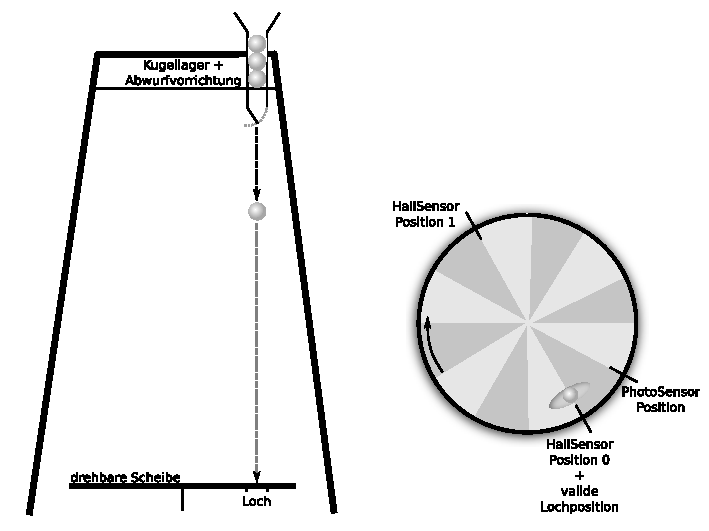
\includegraphics[width=\textwidth]{images/aufbau.pdf}
	\caption{schmatischer Versuchsaufbau - v.\,l.\,n.\,r. Seitenansicht Gesamtaufbau, Drehbare Scheibe}
	\label{img:versuchsaufbau}
\end{figure}

\begin{center}
\begin{tabular}{lc} 
	\textbf{Eigenschaft} 	& \textbf{Beschreibung}	\\
	\toprule
	\multicolumn{2}{c}{Tisch}\\ 
	\midrule
	Abwürfhöhe 	& 750\,mm \\
	\#Schwarzer Felder 	& 6 \\
	\#Weiße Felder 	& 6 \\
	Lochlänge innen 	& 55\,mm \\
	\midrule 
	\multicolumn{2}{c}{Kugel}\\ 
	\midrule
	Masse 	& 8.5\,g \\
	Durchmesser 	& 12\,mm \\
	\bottomrule
\end{tabular}
\end{center}

\subsection{Sensoren}
Der Hallsensor zeigt zwei mal pro Umdrehung exakt die Position der Scheibe an.
Dies geschieht, wenn das Loch an \texttt{HallSensorPosition1} und \texttt{HallSensorPosition0} ist (siehe Abb. \ref{img:versuchsaufbau}), wobei zweiteres der Position entspricht, an welcher die Kugel durch das Loch fallen muss.
An den Positionen wechselt die Ausgabe der Sensoren auf den entsprechenden Wert, daher 1 bzw. 0.

Der Photosensor gibt abhängig davon, ob er eine helle oder dunkle Fläche vor sich hat eine 1 oder 0 aus.
Da die Felder auf der Unterseite der Scheibe gleichmäßig verteilt sind (siehe Abb. \ref{img:versuchsaufbau}), kann er nicht zur Positionsbestimmung, dafür für die Bestimmung der Drehgeschwindigkeit verwendet werden.

Die Sensorwerte für Hall- und Photosensor einer Scheibenumdrehung sind in Abb. \ref{img:sensorwerte} dargestellt.

Der dritte Sensor ist ein Trigger, welcher 1 ausgibt, wenn er gedrückt wird.
Dieser soll dafür benutzt werden den Kugelfall zu initiieren, bzw. die Anzahl der Kugeln zu bestimmen, welche zum nächstmöglichen Zeitpunkt fallen gelassen werden sollen.

\subsection{Aktoren}
\label{subs:aktoren}
Wie bereits beschrieben, wird die Abwurfvorrichtung durch einen Servo gesteuert.
Sobald sich dieser aus seiner Ursprungsposition auf einen Winkel von 30° dreht, fällt eine Kugel aus dem Magazin und die nächste Kugel wird automatisch nachgeladen.

Weiterhin gibt es noch einige LEDs, welche in der Implementierung keine besondere Rolle besitzen.

\subsection{Ansteuerung der Komponenten}
Für das Auslesen der Sensoren und die Ansteuerung der Aktoren stehen ein Arduino UNO und eine Art Blackbox zur Verfügung.
Zweitere sorgt dafür, dass die Sensoren und Aktoren direkt an die Pins des Arduino angeschlossen sind, und einfach mittels \texttt{digitalWrite} und \texttt{digitalRead} angesteuert werden können.
Die Belegung der Pins sind in der folgenden Tabelle beschrieben:


\begin{center}
\begin{tabular}{cll} 
	\textbf{Pin} 	& \textbf{In/Out} & \textbf{Funktion}	\\
	\toprule
	2 &	Input &	Photosensor \\
	3 &	Input &	Hallsensor\\
	4 &	Input &	Trigger\\
	5 &	Input &	Switch\\
	7 &	Output &	Blackbox LED gelb\\
	9 &	Output &	Servo\\
	10 &	Input &	Button 1\\
	11 &	Input &	Button 2\\
	12 &	Output &	LED 1\\
	13 &	Output &	LED 2\\
	\bottomrule
\end{tabular}
\end{center}

\begin{figure}[h] \centering
	\includegraphics[width=\textwidth]{images/generated/sensor_messwerte1.pdf}
	\caption{Sensorzyklus einer Scheibenumdrehung}
	\label{img:sensorwerte}
\end{figure}

\section{Fallzeit der Kugel}
Um die Fallzeit einer Kugel zu berechnen wird die Formel für den freien Fall im homogenen Feld
\begin{align}
	t(h) = \sqrt{\frac{2h}{g}}
\end{align}
verwendet.
Setzt man die oben beschriebenen, am Versuchsaufbau gemessenen, Werte ein
\begin{align}
t(h) &= \sqrt{\frac{2 \cdot 0.75m}{9.81\,\nicefrac{m}{s^2}}} \\
	 &= 0.391\,s \\
	 &= 391\,ms
\end{align}
so kommt man auf eine Fallzeit von 391\,ms für eine Kugel.

\subsection{Drehbewegung der Scheibe}
Der Aufbau der Scheibe wurde bereits beschrieben.
Für eine korrekte Berechnung der Abwurfszeit wird des weiteren eine Beschreibung des Drehverhaltens benötigt.
Bei Messungen konnte folgendes Polynom für die Drehgeschwindigkeit [U/min] über der Zeit [s] (siehe Abb. \ref{img:drehgeschw}) festgestellt werden:
\begin{align}
	f(t) = 151.16 - 1.57 \cdot t + 0.0037 \cdot t^2 \label{form:f(t)}
\end{align}
Umgerechnet in die Funktion für die Zeit [ms] pro Umdrehung ergibt sich:
\begin{align}
	h(t) 	&= \frac{60000}{151.16 - 1.57t + 0.0037 \cdot t^2} \\
	    	&= \frac{1.62162\cdot 10^7}{(t-276.65) (t-147.674)} \label{form:h(t)}
\end{align}
Die Umkehrfunktion, daher die Funktion, um mittels der Zeit pro Umdrehung die Position auf $h(t)$ zu berechnen, lautet:
\begin{align}
	h^{-1}(t) 	= 212.162 \pm \frac{0.27027 \cdot \sqrt{56933\cdot t^2 + 2.22\cdot 10^8 \cdot t}}{t} \label{form:h-1(t)}
\end{align}
Da später die Bremsgeschwindigkeit, daher die Beschleunigung vorausgesagt werden muss die erste Ableitung von $h(t)$ berechnet werden:
\begin{align}
	h'(t) 	= \frac{6.88093\cdot 10^9 - 3.24324 \cdot 10^7 \cdot t}{(t^2 - 424.324\cdot t + 40854.1)^2} \label{form:h'(t)}
\end{align}

% Approximationskurve
\begin{figure}[hb] \centering
	\includegraphics[width=\textwidth]{images/generated/Data2.pdf}
	\caption{Drehgeschwindigkeit über der Zeit approximiert mit der Funktion: \ref{form:f(t)}}
	\label{img:drehgeschw}
\end{figure}

